
\begin{flushleft}

There are two major parts of an L-systems implementation, firstly there is the L-system rewriter, which takes a defined L-system that complies to a partacular grammar, the starting point will be rewritten a number of times using the set of production rules. The rewriting system will give a set of instructions, sometimes called the resultant string. This resultant string is passed to the second system called the interpreter. The interpreter runs through each character or instruction within the resulting string  and interprets its meaning, this acts as a set of instructions that are carried out by turtle graphics to eventually represent a model of a plant on the screen. This chapter will focus on the rewriting system. This includes formaly defining a context-free grammar which the L-system must obide by. Once the grammar has been formalized, a lexical analyser and parser, similar to those used in interpreters and compilers in computing, can be created to represent the context-free L-system grammar, essentially, creating an compiler for a context-free L-system grammar. Using this compiler we can write an L-system, similar to a computer program, the L-system "program" will be passed into the lexical analyser and then through the parser, where each component of the L-system will be identified and parsed into the appropriate computational structures. If the syntax is valid and the parser is successful, the structures created during parsing will be used to rewrite the L-system to a given generation. If the L-system provided does not match the context-free grammar definition, an appropriate error message can be displayed. \\

\vspace{5mm}

For simple D0L-system seen in section \ref{DOL-system example}, creating a rewriter for a simple L-system such as this is quite simple, each rewritable symbol is only made up of a single character, and because the D0L-system is deterministic we know that there is no randomess when determining the matching rule. This is just a case of storing the starting string, and then iterating through this string one character at a time and when a symbol matches that in a rule, replace that character with the string provided by the rule. This can be programmed relatively simply, however, if we are to implement the parametric 0L-system, such as having each instruction be a module with multiple parameters and the parameters being expressions, the rewriting system will have to better understand what each part of the L-system is specifying based on the grammar that it belongs to. The lexical analyser and parser can be used for this purpose in order to classify each part of the L-system and prepare it for rewriting. \\

\vspace{5mm}

For the rewriting system I will be refering to definition of an L-system, the part containing information about the L-system, the axiom and the production rules.  

\end{flushleft}

\section{Environment and Tools}

\begin{flushleft}

This majority of the implementation of the L-system will be written in the C and C++ programming languages \cite{stroustrup2000c++}, and I will be using the modern Open Graphics Library or \gls{OpenGL}. The OpenGl framework is one of the industry standards for creating 3D graphics applications, and is a cross platform API for interacting with the \acrshort{gpu} in a low level way. The low level nature of OpenGL is important as some of the structures and models we are going to be displaying and simulating can be graphically intensive \cite{sellers2013opengl} \cite{movania2017opengl}. OpenGL was originally intended to be an \acrshort{api} for the C and C++ programming languages, and therefore we can have a programming language and graphics API which have a strong emphasis on performance.

\vspace{5mm}

There are also a number of libraries which will provide some extra functionality. The standard library for C and C++ provides many usefull structures and functions which will be incredibly usefull during the development process. For more specialised mathematics capabilities the \acrfull{glm} library holds many mathematics classes and functions for conveniently dealing with some 3D mathematics such as vectors, matrices and quaternions. Another important library is the \acrfull{glfw} which is a multiplatform \acrshort{api} for creating an managing user interface windows, events and user input \cite{glfwDocumentation}.

\vspace{5mm}

In order to keep track of changes and manage versions Git is a free and open source version control software, that is able to keep track of changes that have been made to the files within a project folder. It will be used to keep track of previous versions of the project throughout the development process. Git can be used in conjuction with Github, which is a online web application that stores git repositories. This acts as a backup as well as containing all previous versions of the project \cite{torvalds}.

\end{flushleft}

\section{Formalising the L-system Descriptor}

\section{L-system Generator} \label{l-system generator section}

The purpose of the L-system generator is to read a file, called the L-system discriptor which contains any information that might be necessary for the string rewriting process. This file must contain the number of times the string will be rewritten (number of generations), a starting point (axiom) and at least one production rule, it may also contain some constant variables and other information. \\
\\
For simple L-systems, the generator need not be too complicated. The Koch Curve L-system stated below is a good example of this. \\
\\
\textbf{Angle:} 90\\
\textbf{Axiom:} F\\
\textbf{Rules:} \\
F $\rightarrow$ F+F-F+F\\
\\
Here we have a constant value of 90 degrees, the starting point of 'F' and one rule F $\rightarrow$ F+F-F+F. This type of system is very simple to rewrite computationally. \\ 
\\
\textbf{\textit{Here we describe some pseudocode}}\\

\begin{algorithmic}
\STATE $i \gets 10$
\end{algorithmic}

When we move onto some more complicated L-systems, such as those that use parameters which have expressions with both variables and numbers. We end up with an L-system file that is quite difficult to process and rewrite. In order to compute these complex L-systems we need to first develop a formal grammar that describes how L-system files are defined. Once we have a formalization of how to define an parametric l-system we can create a system to carry out the rewriting.

\section{The Need for a L-system Lexical Analyser and Parser}

Traditionally an interpreter is a program that takes program code as input, where it is then analyzed and interpreted as it is encountered in the execution process. All of the previously encountered information is kept for later interpretations. The information about the program can be extracted by inspection of the program as a whole, such as the set of declared variables in a block, a function, etc \cite{wilhelm2010compiler}. \\
\\
A similarity can be drawn between traditional interpreted languages and the L-system descriptors. With the L-system descriptors we are defining a set of constant variables, a starting point and then some production rules. Once we have all of this information, we would like to interpret that information a number of times. \\
For instance, we may want to rewrite five generations of the L-system, but later on we may want to instead generate up to the tenth generation. So we don't want to have to throw all the previous information away and start from scratch, instead, we can go from the current state of the interpreter and just rewrite another five times. If we would then like to get the resulting string we can just ask for it from the interpreter. \\
\\
To make the most of a \acrshort{cfg} like the L-system grammar, creating an interpreter specifically designed to interpret the L-system descriptors can not only make it simpler to debug any syntactic errors, but also make the string rewriting much faster.\\
\\
In compilers and interpreteres there is usually a three step process in order to understand the input program. The first is the scanner or lexical analyser, the output of the scanner is then processed using the parser, this generates a syntax tree which is then further processed by a context-sensitive analyser. I will be elaborating on each of these processes in sections \ref{Flex} and \ref{Bison}. \\


\subsection{Building a Generalised L-system Grammar}

We are now able to represent complex three dimensional tree structures in the form of a L-system rule set. In a computing sense this rule set can be seen as a type of program. In the program we define the number of generations we would like to generate, the starting point (Axiom) some constant varables (\#define) and the set of production rules. \\
Using this information, we iterate through the from generation to generation rewritting the strings and then at the end provide a resulting string which will then be interpreted and displayed on the screen.
\\
We can represent the languages grammar in the form of a \acrlong{bnf}, \acrshort{bnf} is a notation for \acrlong{cfg}s used to describe the syntax of different languages. In this case the \acrshort{bnf} is used below to describe the syntax of the parametric L-system grammar. \\
\\
For example: \\ 
\\
\textless expression\textgreater~ $\rightarrow$ number \\ 
\textless expression\textgreater~ $\rightarrow$ (\textless expression\textgreater~) \\
\textless expression\textgreater~ $\rightarrow$ \textless expression\textgreater~ + \textless expression\textgreater~ \\
\textless expression\textgreater~ $\rightarrow$ \textless expression\textgreater~ - \textless expression\textgreater~ \\
\\
The first line states that an \textless expression\textgreater~ can be any number, line two states that an \\ \textless expression\textgreater~ can also be an expression that is inside parenthesis. Line three states that an \\ \textless expression\textgreater~ can be an \textless expression\textgreater~ added to another \textless expression\textgreater~, furthermore line four states that an \textless expression\textgreater~ can also be an \textless expression\textgreater~ subtracted by another \textless expression\textgreater~. \\
\\
The above grammar can be expressed as follows: \\
\\
\textless expression\textgreater~ $\rightarrow$ number 

\hspace{2cm} $|$ (\textless expression\textgreater~) 

\hspace{2cm} $|$ \textless expression\textgreater~ + \textless expression\textgreater~ 

\hspace{2cm} $|$ \textless expression\textgreater~ - \textless expression\textgreater~ \\
\\
Here the $|$ symbol can be articulated as an OR, therefore it can be said that an \textless expression\textgreater~ can be a number OR an \textless expression\textgreater~ surrounded by parenthesis, OR an \textless expression\textgreater~ added to another \textless expression\textgreater~ OR an \textless expression\textgreater~ subtracted by another \textless expression\textgreater~. 
\\
In addition to this, any statement that is not surrounded by \textless \textgreater, states it must match that particular string. The $\in$ followed by an $|$ states that it can either be nothing or another statement. \\
\\


\newpage 
\subsection{\acrlong{bnf} of the L-system Grammar} \label{L-system Grammar}

% Program 
\noindent
\textless prog\textgreater~ $\rightarrow$ $\in$ 

\hspace{2cm} $|$  \textless stmts\textgreater~ EOF \\



% Statements
\noindent
\textless stmts\textgreater~ $\rightarrow$ $\in$

\hspace{2cm} $|$ \textless stmt\textgreater~ \textless stmts\textgreater~ \\


% Statement
\noindent
\textless stmt\textgreater~ $\rightarrow$ EOL 

\hspace{2cm} $|$ \textless generations\textgreater~

\hspace{2cm} $|$ \textless definition\textgreater~

\hspace{2cm} $|$ \textless axiom\textgreater~

\hspace{2cm} $|$ \textless production\textgreater~\\



% Generations
\noindent
\textless generations\textgreater~ $\rightarrow$ \#n = \textless float\textgreater~ ; \\



% Definitions
\noindent
\textless definition\textgreater~ $\rightarrow$  \#define \textless variable\textgreater~ \textless float\textgreater~ ;

\hspace{2cm} $|$ \#define \textless variable\textgreater~ + \textless float\textgreater~ ;

\hspace{2cm} $|$ \#define \textless variable\textgreater~ -\textless float\textgreater~ ; \\



% Axiom
\noindent
\textless axiom\textgreater~ $\rightarrow$  \#w : \textless axiom statement list\textgreater~ ; \\



% Axiom Statement List
\noindent
\textless axiom statement list\textgreater~ $\rightarrow$ $\in$ 

\hspace{2cm} $|$ \textless axiom statement\textgreater~ \textless axiom statement list\textgreater~ ; \\



% Axiom Statement
\noindent
\textless axiom statement\textgreater~ $\rightarrow$ \textless moduleAx\textgreater~ \\



% Axiom Module 
\noindent
\textless moduleAx\textgreater~  $\rightarrow$ \textless variable\textgreater~ $|$ "$+$" $|$ "$-$" $|$ "/" $|$ "$\backslash$" $|$ "\textasciicircum" $|$ "$\&$" $|$ "!" 

\hspace{2cm} $|$ \textless variable\textgreater~ (  \textless paramAx\textgreater~ \textless paramListAx\textgreater~ )

\hspace{2cm} $|$ +(  \textless paramAx\textgreater~ \textless paramListAx\textgreater~ ) 

\hspace{2cm} $|$ -(  \textless paramAx\textgreater~ \textless paramListAx\textgreater~ ) 

\hspace{2cm} $|$ /(  \textless paramAx\textgreater~ \textless paramListAx\textgreater~ ) 

\hspace{2cm} $|$ $\backslash$(  \textless paramAx\textgreater~ \textless paramListAx\textgreater~ )

\hspace{2cm} $|$ \textasciicircum (  \textless paramAx\textgreater~ \textless paramListAx\textgreater~ ) 

\hspace{2cm} $|$ $\&$(  \textless paramAx\textgreater~ \textless paramListAx\textgreater~ ) \\



% Axiom Parameter List
\noindent
\textless paramAxList\textgreater~ $\rightarrow$  $\in$ 

\hspace{2cm} $|$ , \textless paramAx\textgreater~ \textless paramAxList\textgreater~ \\



% Axiom Parameter
\noindent
\textless paramAx\textgreater~ $\rightarrow$ \textless expression\textgreater~ \\



% Production
\noindent
\textless production\textgreater~ $\rightarrow$  \# \textless variable\textgreater~  : \textless predecessor\textgreater~ : \textless condition\textgreater~  : \textless successor\textgreater~ ;\\



% Predecessor
\noindent
\textless predecessor\textgreater~ $\rightarrow$ \textless pred statement list\textgreater~ \\


% Predecessor Statement List
\noindent
\textless pred statement list\textgreater~ $\rightarrow$ $\in$

\hspace{2cm} $|$ \textless pred statement\textgreater~ \textless pred statement list\textgreater~ \\


% Predecessor Statement
\noindent
\textless pred statement\textgreater~ $\rightarrow$ \textless module\textgreater~ \\



% Condition 
\noindent
\textless condition\textgreater~ $\rightarrow$ *

\hspace{2cm} $|$ \textless left expression\textgreater~ \textless conditions statement\textgreater~ \textless right expression\textgreater~ \\


% Condition Left Expression
\noindent
\textless left expression\textgreater~ $\rightarrow$ \textless expression\textgreater~ \\


% Condition Right Expression
\noindent
\textless right expression\textgreater~ $\rightarrow$ \textless expression\textgreater~ \\


% Condition Statement
\noindent
\textless condition statement\textgreater~ $\rightarrow$ == $|$ != $|$ \textless $|$ \textgreater $|$ \textless = $|$ \textgreater =\\



% Successor
\noindent
\textless successor \textgreater~ $\rightarrow$ \textless successor statement list \textgreater~ \\


% Successor Statement List
\noindent
\textless successor statement list\textgreater~ $\rightarrow$ $\in$

\hspace{2cm} $|$ \textless successor statement\textgreater~ \textless successor statement list \textgreater~ \\


%Successor Statement
\noindent
\textless successor statement\textgreater~ $\rightarrow$ \textless module\textgreater~ \\



% Module
\noindent
\textless module\textgreater~ $\rightarrow$  \textless variable\textgreater~ $|$ $+$ $|$ $-$ $|$ / $|$ $\backslash$ $|$ \textasciicircum $|$ $\&$ $|$ ! 

\hspace{2cm} $|$ \textless variable\textgreater~ (  \textless param\textgreater~ \textless paramList\textgreater~ )

\hspace{2cm} $|$ +(  \textless param\textgreater~ \textless paramList\textgreater~ )

\hspace{2cm} $|$ -(  \textless param\textgreater~ \textless paramList\textgreater~ )

\hspace{2cm} $|$ /(  \textless param\textgreater~ \textless paramList\textgreater~ ) 

\hspace{2cm} $|$ $\backslash$(  \textless param\textgreater~ \textless paramList\textgreater~ ) 

\hspace{2cm} $|$ \textasciicircum (  \textless param\textgreater~ \textless paramList\textgreater~ ) 

\hspace{2cm} $|$ $\&$(  \textless param\textgreater~ \textless paramList\textgreater~ ) \\



% Parameter List
\noindent
\textless paramList\textgreater~ $\rightarrow$ $\in$ $|$ : \textless param\textgreater~ \textless paramList\textgreater~ \\



%Parameter List
\noindent
\textless param\textgreater~ $\rightarrow$ \textless expression\textgreater~ \\



% Expression
\noindent
\textless expression\textgreater~ $\rightarrow$  \textless variable\textgreater~

\hspace{2cm} $|$ \textless float\textgreater~

\hspace{2cm} $|$ \textless expression\textgreater~ + \textless expression\textgreater~

\hspace{2cm} $|$ \textless expression\textgreater~ - \textless expression\textgreater~

\hspace{2cm} $|$ \textless expression\textgreater~ * \textless expression\textgreater~

\hspace{2cm} $|$ \textless expression\textgreater~ / \textless expression\textgreater~

\hspace{2cm} $|$ \textless expression\textgreater~ \textasciicircum \textless expression\textgreater~

\hspace{2cm} $|$ "(" \textless expression\textgreater~ ) \\



% Float
\noindent
\textless float\textgreater~ $\rightarrow$ [0-9]+.[0-9]+ \\



% Variable
\noindent
\textless variable\textgreater~ $\rightarrow$ [a-zA-Z\_][a-zA-Z0-9\_]* \\


\subsection{Scanner - Flex} \label{Flex}

D. Cooper and L. Torczon write that "The scanner, or lexical analyser, reads a stream of characters and produces a streeam of words. It aggregates characters to form words and applies a set of rules to determin wheter or not each word is legal in the source language. If the word is valid, the scanner assigns it a syntactic category, or part of speech" \cite{cooper2011engineering}. \\
\\ 
Writing a custom \gls{Lexer} can be quite complicated and time consuming to design and implement, and once a custom \gls{Lexer} has been created it can be difficult to change some functionality at a later stage. Luckely there is a well known program known as the \acrlong{flex} (\acrshort{flex}), \acrshort{flex} takes a .lex file which contains the lexical rules of the language, it uses these rules to create a \gls{Lexer} program. When \acrshort{flex} is run it will create a \gls{Lexer} in the form of a C program. \\
\\    


\subsection{Parser - Bison} \label{Bison}

The parsers job is to find out if the input stream of words from the \gls{Lexer} makes up a valid sentence in the language. The \gls{Parser} fits the syntactical category to the grammatical model of the language. If the \gls{Parser} is able to fit the syntactical category of the word to the grammatical model of the language then the syntax is seen to be correct. If all of the syntax is correct the \gls{Parser} will output a syntax tree and build the structures for use later on during the compilation process \cite{cooper2011engineering}.




\section{Displaying the L-system Instructions} \label{Display L-system Instructions}

\subsection{Basic 2D L-systems} 

There are a number of fractal geometry that have become well known particularly with regards to how they can seemingly imitate nature \cite{mandelbrot1982fractal}. Particularly with the geometry such as the Koch snowflake which can be represented using the following L-system.

\begin{figure}[htbp]
	\raggedright
	\textbf{\underline{Koch Curve:}} \\
	\#n = 4; \\
	\#define r 90; \\
	\#w : F(1); \\
	\#p1 : F(x) : * : F(x)+(r)F(x)-(r)F(x)-(r)F(x)+(r)F(x);\\
	{\centering
		\vspace{7px}
		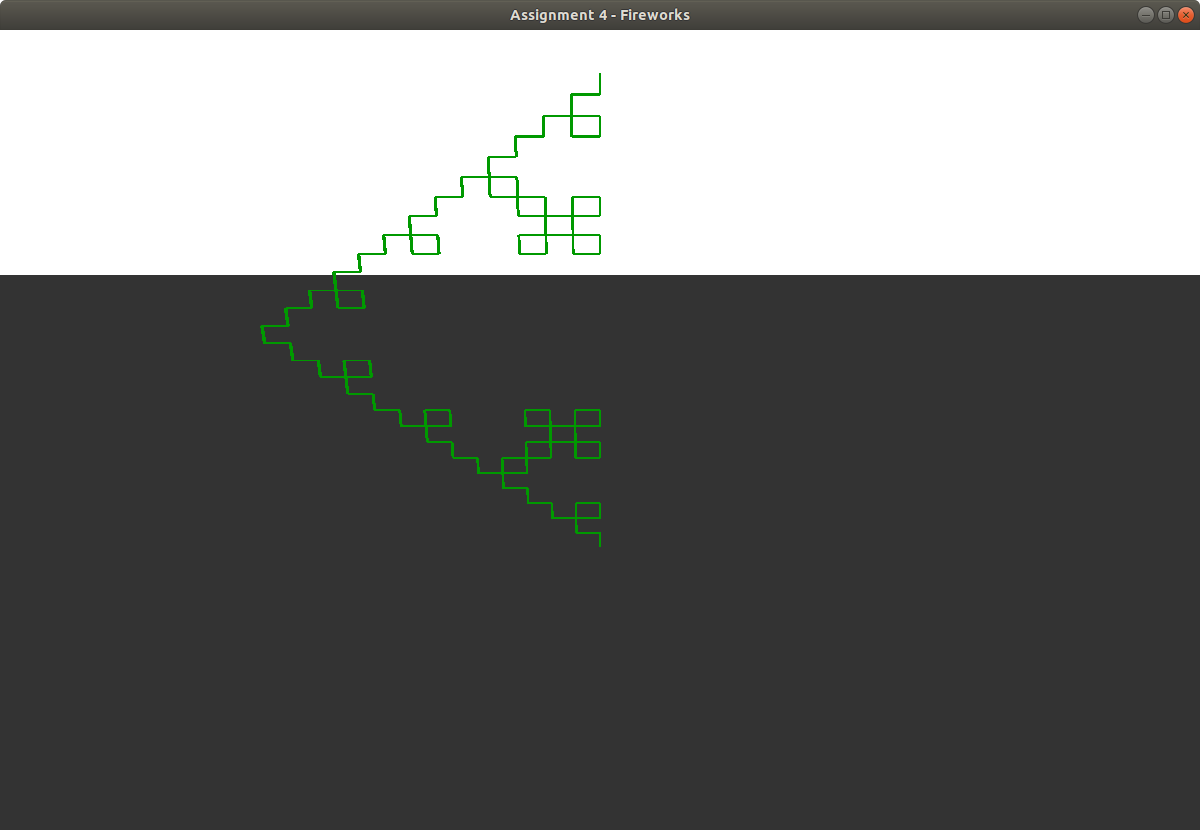
\includegraphics[scale=0.15]{KochCurve/KochCurve04.png}
		\caption{Koch Curve.}
	}
\end{figure}
\begin{figure}[htbp]
	\raggedright
	\textbf{\underline{Sierpinski Triangle:}} \\
	\#n = 4;\\
	\#define r 60;\\
	\#w : F(1);\\
	\#p1 : F(x) : * : X(x)-(r)F(x)-(r)X(x);\\
	\#p2 : X(x) : * : F(x)+(r)X(x)+(r)F(x);\\
	{\centering
		\vspace{7px}
		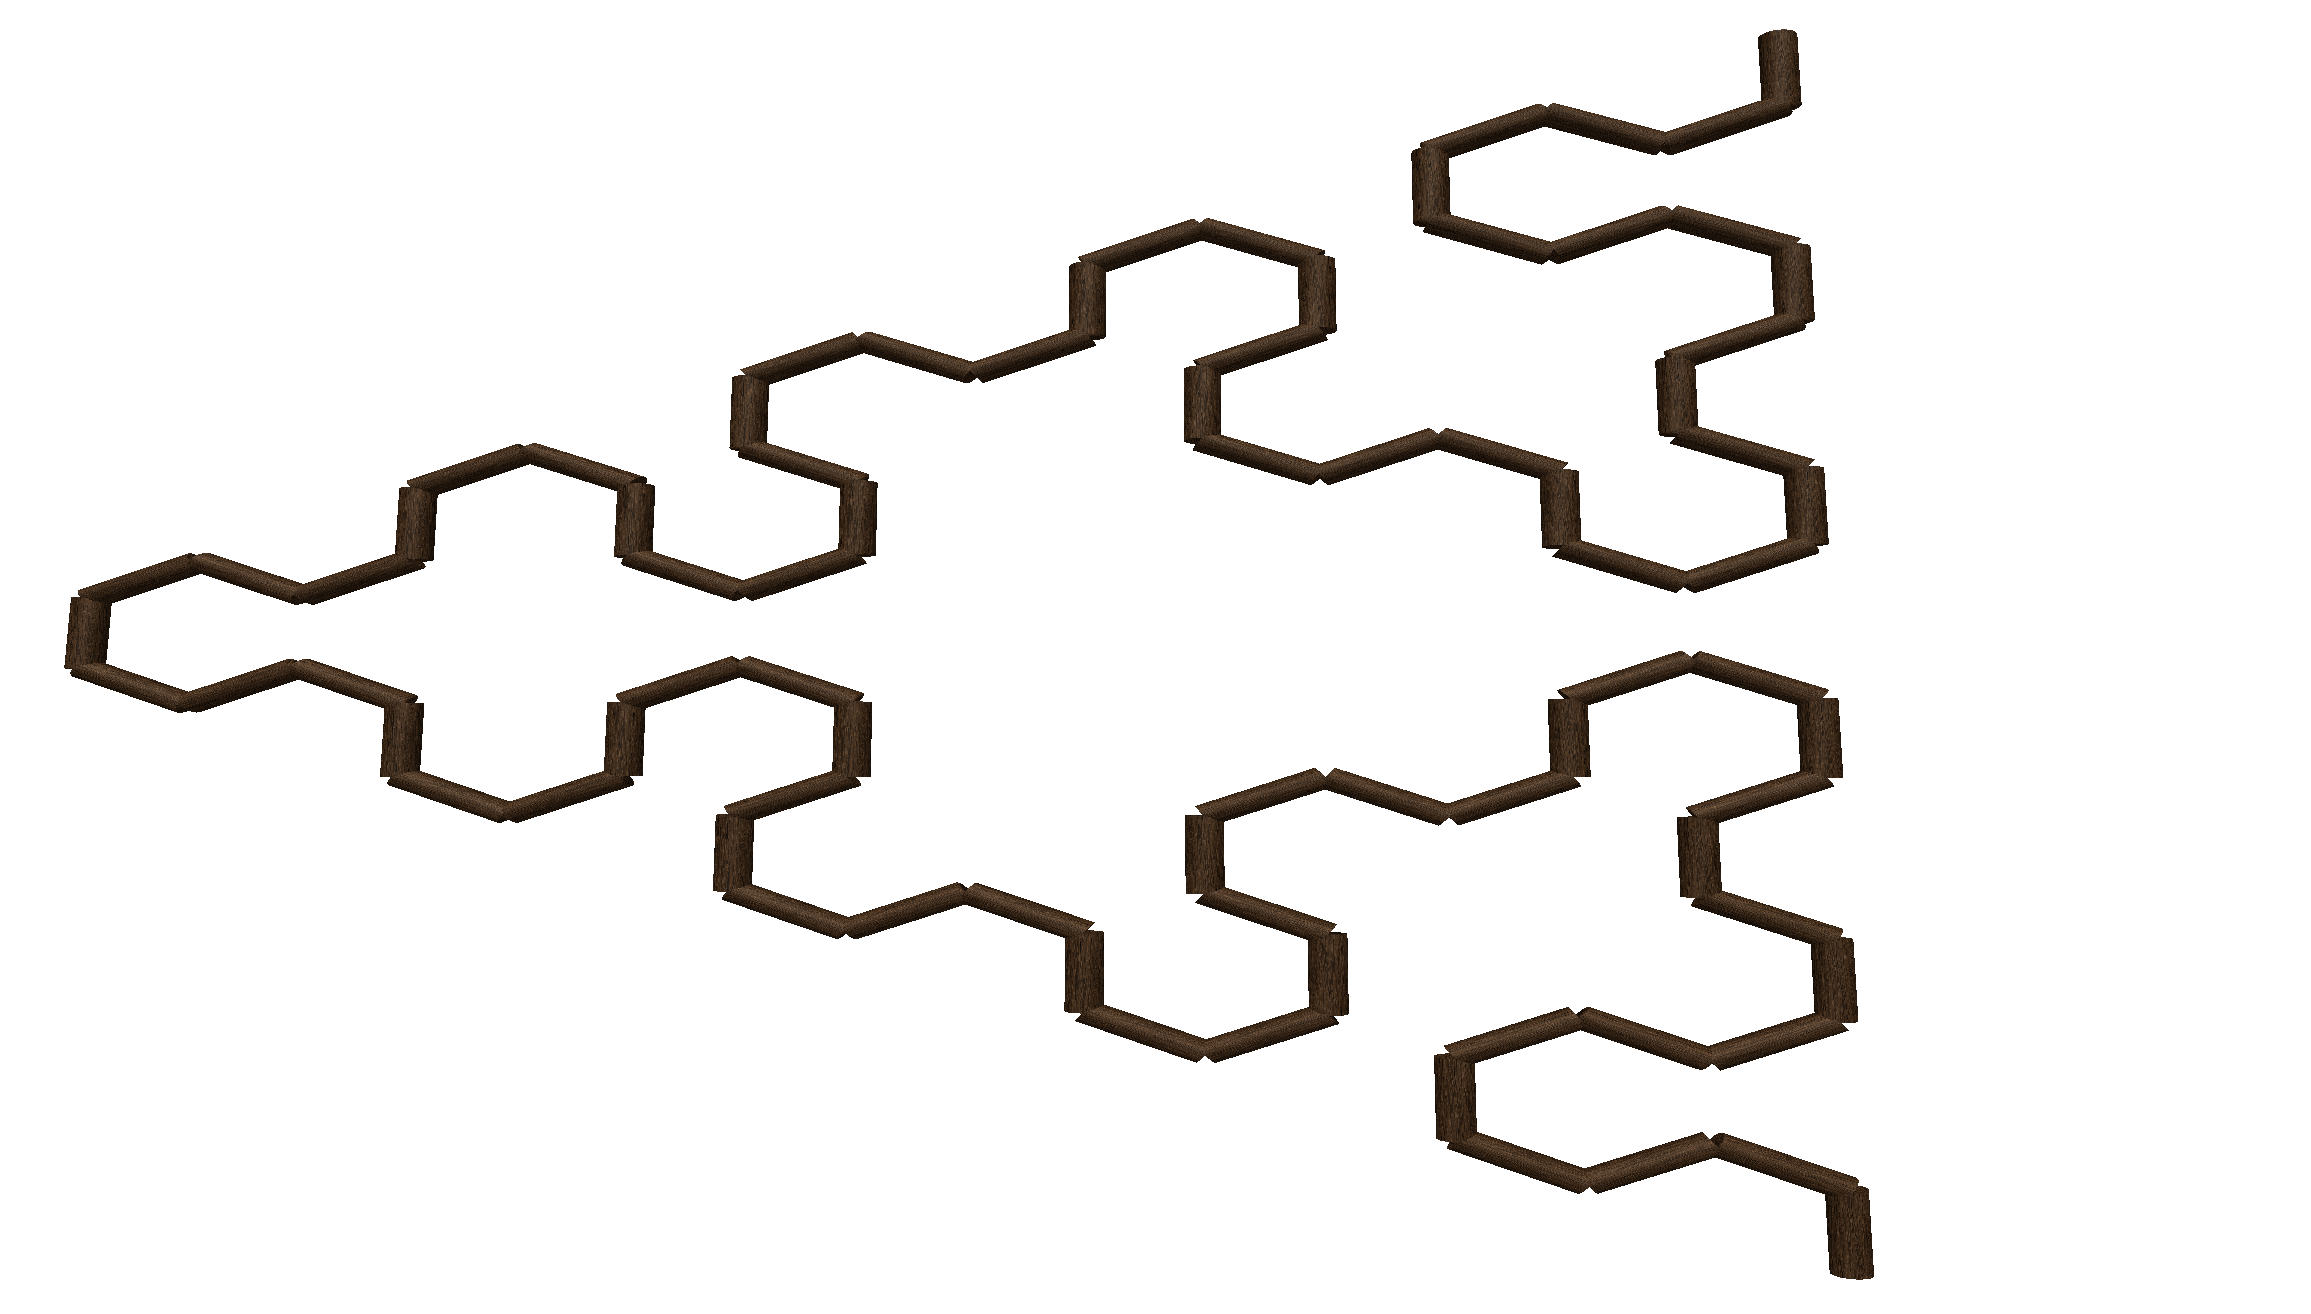
\includegraphics[scale=0.15]{SierpinskiTriangle/SierpinskiTriangle04.png}
		\caption{Sierpinski Triangle.}
	}
\end{figure}
\begin{figure}[htbp]
	\raggedright
	\textbf{\underline{Fractal Plant:}} \\
	\textbf{Alphabet:} X, F\\
	\textbf{Constants:} +, -, [, ] \\
	\textbf{Axiom:} X \\
	\textbf{Angle:} 25$^\circ$ \\
	\textbf{Rules:} \\
	X $\rightarrow$ F-[[X]+X]+F[+FX]-X\\
	F $\rightarrow$ FF \\
	{\centering
		\vspace{7px}
		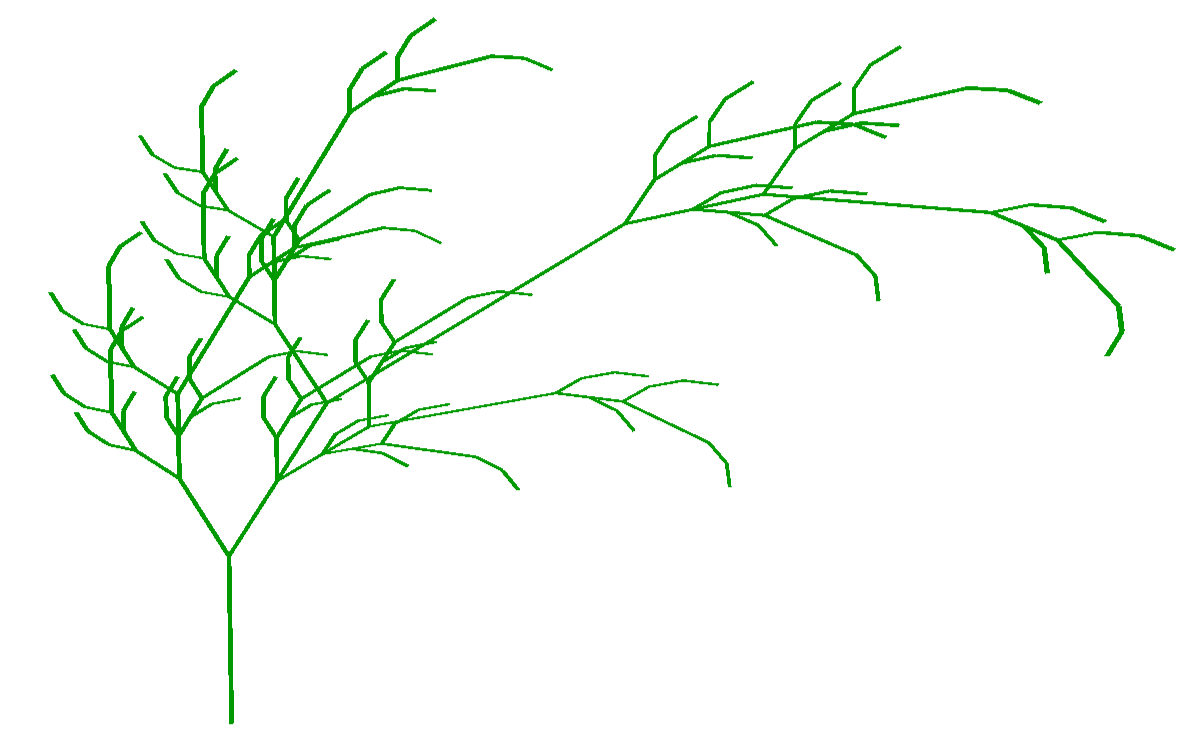
\includegraphics[scale=0.15]{FractalPlant/FractalPlant05.png}
		\caption{Fractal Plant.}
	}
\end{figure}
\begin{figure}[htbp]
	\raggedright
	\textbf{\underline{Fractal Bush:}} \\
	\textbf{Alphabet:} F\\
	\textbf{Constants:} +, -, [, ] \\
	\textbf{Axiom:} F \\
	\textbf{Angle:} 25$^\circ$ \\
	\textbf{Rules:} \\
	F $\rightarrow$ FF+[+F-F-F]-[-F+F+F]\\
	{\centering
		\vspace{7px}
		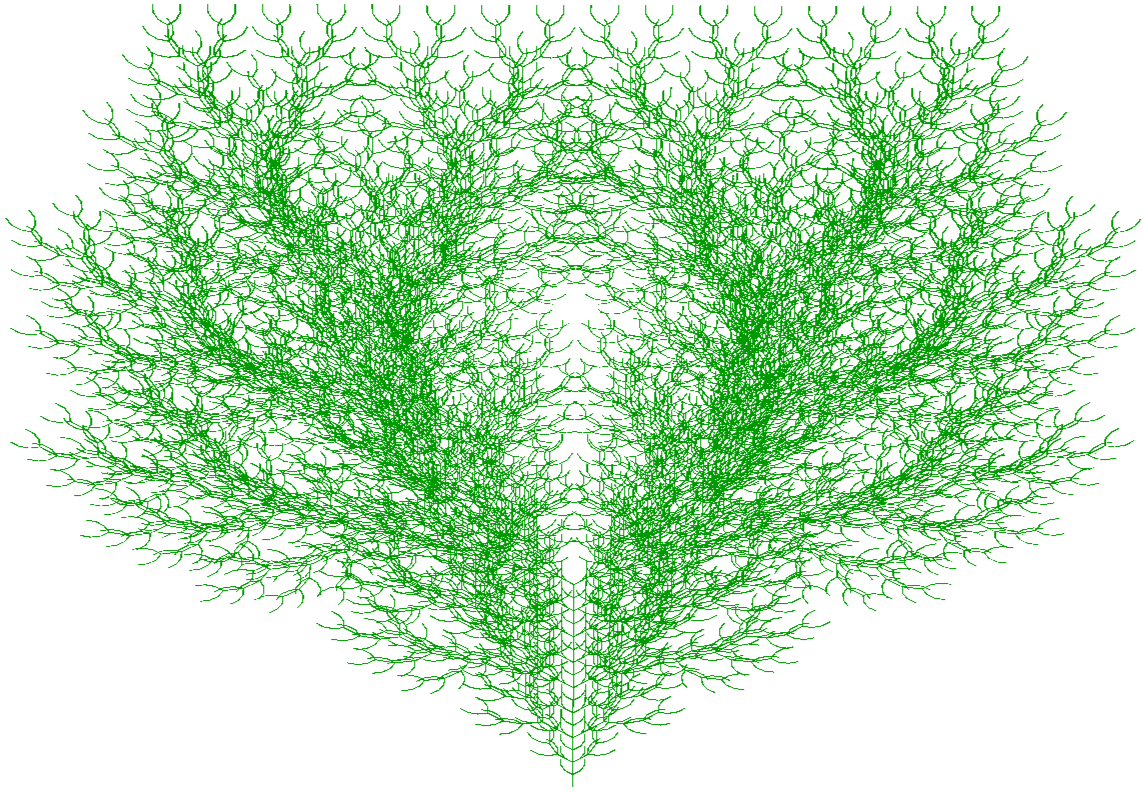
\includegraphics[scale=0.15]{FractalBush/FractalBush06.png}
		\caption{Fractal Bush.}
	}
\end{figure}

\FloatBarrier

\subsection{The Use of L-systems in 3D applications}

\begin{flushleft}

L-systems have been talked about and researched since its inception in 1968 by Aristid Lindenmayer. Over the years it's usefulness in modelling different types of plant life has been very clear, however its presence has been quite absent from any mainstream game engines for the most part, these engines relying either on digital artists skill to develop individual plants or on 3rd party software such as SpeedTree. These types of software use a multitude of different techniques however their methods are heavily rooted in Lindenmayer Systems. 

\end{flushleft}

\newpage